% Options for packages loaded elsewhere
\PassOptionsToPackage{unicode}{hyperref}
\PassOptionsToPackage{hyphens}{url}
\PassOptionsToPackage{dvipsnames,svgnames,x11names}{xcolor}
%
\documentclass[
  10pt,
]{article}
\usepackage{amsmath,amssymb}
\usepackage{iftex}
\ifPDFTeX
  \usepackage[T1]{fontenc}
  \usepackage[utf8]{inputenc}
  \usepackage{textcomp} % provide euro and other symbols
\else % if luatex or xetex
  \usepackage{unicode-math} % this also loads fontspec
  \defaultfontfeatures{Scale=MatchLowercase}
  \defaultfontfeatures[\rmfamily]{Ligatures=TeX,Scale=1}
\fi
\usepackage{lmodern}
\ifPDFTeX\else
  % xetex/luatex font selection
\fi
% Use upquote if available, for straight quotes in verbatim environments
\IfFileExists{upquote.sty}{\usepackage{upquote}}{}
\IfFileExists{microtype.sty}{% use microtype if available
  \usepackage[]{microtype}
  \UseMicrotypeSet[protrusion]{basicmath} % disable protrusion for tt fonts
}{}
\makeatletter
\@ifundefined{KOMAClassName}{% if non-KOMA class
  \IfFileExists{parskip.sty}{%
    \usepackage{parskip}
  }{% else
    \setlength{\parindent}{0pt}
    \setlength{\parskip}{6pt plus 2pt minus 1pt}}
}{% if KOMA class
  \KOMAoptions{parskip=half}}
\makeatother
\usepackage{xcolor}
\usepackage[margin=0.9in]{geometry}
\usepackage{longtable,booktabs,array}
\usepackage{calc} % for calculating minipage widths
% Correct order of tables after \paragraph or \subparagraph
\usepackage{etoolbox}
\makeatletter
\patchcmd\longtable{\par}{\if@noskipsec\mbox{}\fi\par}{}{}
\makeatother
% Allow footnotes in longtable head/foot
\IfFileExists{footnotehyper.sty}{\usepackage{footnotehyper}}{\usepackage{footnote}}
\makesavenoteenv{longtable}
\usepackage{graphicx}
\makeatletter
\def\maxwidth{\ifdim\Gin@nat@width>\linewidth\linewidth\else\Gin@nat@width\fi}
\def\maxheight{\ifdim\Gin@nat@height>\textheight\textheight\else\Gin@nat@height\fi}
\makeatother
% Scale images if necessary, so that they will not overflow the page
% margins by default, and it is still possible to overwrite the defaults
% using explicit options in \includegraphics[width, height, ...]{}
\setkeys{Gin}{width=\maxwidth,height=\maxheight,keepaspectratio}
% Set default figure placement to htbp
\makeatletter
\def\fps@figure{htbp}
\makeatother
\setlength{\emergencystretch}{3em} % prevent overfull lines
\providecommand{\tightlist}{%
  \setlength{\itemsep}{0pt}\setlength{\parskip}{0pt}}
\setcounter{secnumdepth}{5}
% definitions for citeproc citations
\NewDocumentCommand\citeproctext{}{}
\NewDocumentCommand\citeproc{mm}{%
  \begingroup\def\citeproctext{#2}\cite{#1}\endgroup}
\makeatletter
 % allow citations to break across lines
 \let\@cite@ofmt\@firstofone
 % avoid brackets around text for \cite:
 \def\@biblabel#1{}
 \def\@cite#1#2{{#1\if@tempswa , #2\fi}}
\makeatother
\newlength{\cslhangindent}
\setlength{\cslhangindent}{1.5em}
\newlength{\csllabelwidth}
\setlength{\csllabelwidth}{3em}
\newenvironment{CSLReferences}[2] % #1 hanging-indent, #2 entry-spacing
 {\begin{list}{}{%
  \setlength{\itemindent}{0pt}
  \setlength{\leftmargin}{0pt}
  \setlength{\parsep}{0pt}
  % turn on hanging indent if param 1 is 1
  \ifodd #1
   \setlength{\leftmargin}{\cslhangindent}
   \setlength{\itemindent}{-1\cslhangindent}
  \fi
  % set entry spacing
  \setlength{\itemsep}{#2\baselineskip}}}
 {\end{list}}
\usepackage{calc}
\newcommand{\CSLBlock}[1]{\hfill\break\parbox[t]{\linewidth}{\strut\ignorespaces#1\strut}}
\newcommand{\CSLLeftMargin}[1]{\parbox[t]{\csllabelwidth}{\strut#1\strut}}
\newcommand{\CSLRightInline}[1]{\parbox[t]{\linewidth - \csllabelwidth}{\strut#1\strut}}
\newcommand{\CSLIndent}[1]{\hspace{\cslhangindent}#1}
\ifLuaTeX
  \usepackage{selnolig}  % disable illegal ligatures
\fi
\usepackage{bookmark}
\IfFileExists{xurl.sty}{\usepackage{xurl}}{} % add URL line breaks if available
\urlstyle{same}
\hypersetup{
  pdftitle={RecursiveCal: Reproducible Diagnostic Selection under Model Mismatch},
  pdfauthor={Venkateshwar Reddy},
  colorlinks=true,
  linkcolor={black},
  filecolor={Maroon},
  citecolor={Blue},
  urlcolor={blue},
  pdfcreator={LaTeX via pandoc}}

\title{RecursiveCal: Reproducible Diagnostic Selection under Model
Mismatch}
\author{Venkateshwar Reddy}
\date{Working draft, 21 November 2026}

\begin{document}
\maketitle
\begin{abstract}
Choosing a diagnostic experiment can reduce calibration error, but an
adaptive policy can also act on a misspecified model. RecursiveCal
provides an open source workbench and a reproducible synthetic study of
this distinction. The diagnostic task fixes the first probe and allows
an observation-dependent second probe or stopping, followed by a
discrete calibration decision. We compare fixed schedules, Bayesian
experimental design, a small learned contextual bandit,
matched-frequency shuffled controls, and a mismatch-triggered fallback.
Five learned training seeds are evaluated on 512 shared cases in each of
five cohorts. Under the constructed finite prior, adaptive Bayesian
selection improves mean cost-adjusted reward over the selected fixed
schedule by 0.01233, with a paired 95\% interval of {[}0.01039,
0.01415{]}. A directional-friction structural shift reverses that
comparison: the adaptive method loses 0.00992 {[}0.00496, 0.01530{]}.
The five-seed learned mean is close to the Bayesian result in
distribution, without an established superiority claim. A separate
physical-unit liftgate model supplies numerical verification, explicit
passive-support failures, and a measured-data ingestion path. Its
default coefficients and included examples remain synthetic. The
contribution is an executable research instrument with inspectable
assumptions and negative controls, not a validated hardware controller
or a new general-purpose reinforcement-learning algorithm.
\end{abstract}

\section{Motivation and contribution}\label{motivation-and-contribution}

Calibration combines estimation with a decision about which measurement
is worth acquiring. A diagnostic action can improve the final parameter
choice, consume time or energy, or provide misleading evidence when the
inference model is incomplete. A high average reward by itself does not
establish that a policy learned to adapt its experiments. A fixed test
can perform well on a restricted fault distribution, and a learned
strategy can exploit assumptions that disappear outside that
distribution.

RecursiveCal addresses this evaluation problem with executable controls
and retained trial evidence. Its earlier neural pilot selected the same
diagnostic probe on every reported held-out case. A fixed policy
choosing that probe reproduced the rewards. That negative result
motivated a deliberately observation-dependent task and stronger
controls, rather than a claim of successful adaptive learning from the
earlier scores.

The present release contributes three connected artifacts. First, it
implements a restricted diagnostic benchmark with classical and learned
policies, explicit costs, parameter and structural shifts, frozen
train/validation/test streams, and checkpoint replay. Second, it
provides a separate single-axis liftgate model in SI units with
numerical verification and visible model-adequacy failures. Third, it
implements a local workbench, strict CSV contracts, provenance-bearing
force fitting, trajectory comparison, and versioned exports. These are
software contributions and an exploratory empirical study. No novelty
claim is made for the underlying learning or Bayesian design algorithms.

The experimental design follows the broader emphasis on sound baselines,
selection procedures, uncertainty, and implementation sensitivity
discussed by Patterson et al. (2024). Agarwal et al. (2021) likewise
motivate reporting uncertainty rather than only point estimates. Those
works guide evaluation practice; they do not establish the fidelity or
significance of this particular simulator.

\section{Diagnostic decision problem}\label{diagnostic-decision-problem}

The normalized plant has hidden parameters for motor effectiveness,
friction, load, damping, sensor bias, and a torque deadzone. The scalar
reference implementation is retained from the earlier benchmark. Its
acceleration is

\[
\ddot x = m\,\operatorname{sgn}(u)\max(0,|u|-d)
          - f\tanh(\dot x/0.035)-b\dot x
          -\ell\sin(\pi x/1.1).
\]

Here the variables and coefficients are normalized synthetic quantities,
not the SI liftgate parameters. Six pulse probes use specified torques
and fixture positions. A seventh reference measurement observes sensor
bias. Pulse measurements contain displacement and final velocity with
independent Gaussian noise of standard deviations 0.004 and 0.009. The
reference measurement has standard deviation 0.006. Pulse displacements
do not independently identify sensor bias, so the reference can change
the terminal calibration choice.

The terminal action selects one of 150 legal calibrations. The simulator
evaluates that choice on four fixed motion trajectories. Quality is an
exponential transformation of the reference loss, which includes
tracking, effort, final error, and numerical limit interventions. The
recorded objective is

\[R=Q-0.012C,\]

where \(C\) is diagnostic cost. A pulse costs 1.0 and the reference
costs 1.5. At most two distinct tests can be used. The host evaluator
owns true parameters and reward tables; action methods receive observed
features only.

The task is deliberately short horizon. Adaptive methods share a low
positive first pulse, then choose STOP or one of the six remaining
probes. The final calibrator is common to the policies: it chooses the
legal calibration with highest posterior expected quality under a
ten-model bank. This isolates the second-test decision sufficiently to
implement strong controls, but excludes adaptive choice of the first
probe and longer diagnostic sequences.

The prior contains ten equiprobable synthetic hypotheses spanning
nominal behavior, sensor bias, weak motor, high friction, and deadzone.
Their complete parameter arrays are recorded in the run manifest. They
were constructed to make different follow-up tests useful for different
first observations. This design should not be mistaken for an empirical
distribution of industrial faults.

\section{Experimental method}\label{experimental-method}

\subsection{Data separation and evaluation
cohorts}\label{data-separation-and-evaluation-cohorts}

The release run uses 1,024 training contexts, 512 validation contexts,
and 512 cases in each of five test cohorts. Distinct deterministic
random streams identify the partitions. Every policy receives the same
generated observations for each evaluation case. Saved episode
identifiers include partition, seed, and index.

Finite-prior test cases reuse the ten latent plant types with new
observation noise. Thus their plant support intentionally overlaps
training; this is a new-noise test, not unseen-plant validation.
Continuous jitter perturbs parameters under the same equations. The
high-load and extreme-deadzone cohorts extend specified parameter ranges
absent from the prior. The fifth cohort changes the equations:
positive-velocity friction is multiplied by \(1+a\) for \(a\) uniformly
distributed between 0.5 and 1.2, while negative-velocity friction
remains unchanged. This breaks the reference model's mirror symmetry.
The inference bank remains symmetric.

The structural shift affects both probe observations and terminal
quality. It is a specified synthetic stress case, not an observed real
failure distribution. Exact seeds, ranges, noise, candidate
calibrations, and model arrays are retained with the evidence.

This study is exploratory. Earlier outcomes and development smoke tests
were inspected while constructing the software. In the final runner,
schedule selection, mismatch threshold, and learned checkpoints are
fixed before test generation, but that execution order does not make an
iteratively developed public benchmark independently preregistered or
blinded.

\subsection{Classical policies and cost
controls}\label{classical-policies-and-cost-controls}

The no-probe policy selects the prior-optimal calibration without
collecting data. It is not necessarily a factory setting or an unchanged
deployed controller. The fixed-schedule method ranks 29 zero-, one-, and
two-test schedules on training contexts, then selects among the best
five on validation. The selected schedule is the low positive pulse
followed by the sensor reference. A separate forced-two fixed control is
retained.

The adaptive Bayesian policy evaluates the expected terminal quality
after each permitted second action, subtracts its test cost, and
compares it with stopping. A tensor-product Gauss-Hermite rule
integrates the Gaussian observation likelihood under the finite
posterior. The primary full run uses order 15. Orders 5 and 9 are
recorded for sensitivity, and validation resolution results are saved.
This is a numerical approximation to expected utility, not an exact
continuous-observation optimum. Small differences from learned policies
should be interpreted in light of that approximation.

The forced-two Bayesian control removes STOP. Equal probe counts do not
imply equal total cost because the reference is more expensive. We
therefore retain quality, cost, number of probes, and net reward
separately. An additional shuffled control permutes a policy's chosen
second actions across test cases and recomputes the posterior using each
case's assigned measurement. It preserves aggregate action frequencies
and total diagnostic cost while breaking the observation-action
association. Individual paired cases can still have different costs.

\subsection{Learned policy}\label{learned-policy}

The learned method is a contextual bandit with finite-context replay.
Its input has twelve features: two scaled observed pulse readings and
ten scaled posterior weights. A 48-unit tanh layer maps these features
to seven action values. Training uses Adam with learning rate 0.0015,
700 minibatch updates, and epsilon-greedy exploration decreasing from
0.55 to 0.10. The chosen action's reward is scaled as \((R-0.8)10\) for
squared-error regression.

The host precomputes reward tables for computational efficiency, but
only the selected action's target enters each gradient update. Repeated
visits to one context can sample different action rewards. This is not
fresh online hardware interaction. Every 50 updates, validation reward
is evaluated; the highest validation mean selects the checkpoint, with
earlier checkpoints winning ties. Five independent learner seeds are
retained: 13, 37, 103, 211, and 509.

Checkpoints are saved as JSON weights and reloaded before evaluation.
Artifact verification reconstructs features from saved first
observations and reproduces the selected learned actions.
Information-boundary tests alter hidden parameters, reward tables, and
unobserved probe values while checking that a fixed policy's actions and
observed-data posterior decisions remain unchanged.

\subsection{Mismatch fallback and
uncertainty}\label{mismatch-fallback-and-uncertainty}

The mismatch statistic is the minimum noise-standardized distance
between the first observation and any prior prediction. Its threshold is
the higher empirical 95th percentile on validation contexts, fixed
before test generation. A flagged case stops and uses the prior-optimal
calibration, paying for the first test already performed. This is an
explicit fallback policy, not a certified safeguard or a guaranteed
known-good controller.

Unshuffled policy contrasts use paired case differences with 2,000
percentile bootstrap resamples. Their 95\% intervals condition on a
particular fitted policy and the specified synthetic population. They
exclude uncertainty from choosing the benchmark, physics assumptions,
and hyperparameter development. Learned seed means and their sample
standard deviation are reported separately. Five seeds do not justify
broad claims about training reliability.

Single-permutation shuffled controls are descriptive. Their rows share
an action permutation, so ordinary independent-row bootstrap intervals
would omit dependence and permutation uncertainty. The released summary
explicitly records null inferential intervals for those contrasts.
Multiple policy and cohort comparisons are exploratory, without a
familywise multiplicity correction.

\section{Diagnostic results}\label{diagnostic-results}

Table 1 reports mean net reward. The learned column averages the five
trained seed means, rather than treating all seed-by-episode outcomes as
independent training runs.

\begin{longtable}[]{@{}
  >{\raggedright\arraybackslash}p{(\columnwidth - 10\tabcolsep) * \real{0.1667}}
  >{\raggedleft\arraybackslash}p{(\columnwidth - 10\tabcolsep) * \real{0.1667}}
  >{\raggedleft\arraybackslash}p{(\columnwidth - 10\tabcolsep) * \real{0.1667}}
  >{\raggedleft\arraybackslash}p{(\columnwidth - 10\tabcolsep) * \real{0.1667}}
  >{\raggedleft\arraybackslash}p{(\columnwidth - 10\tabcolsep) * \real{0.1667}}
  >{\raggedleft\arraybackslash}p{(\columnwidth - 10\tabcolsep) * \real{0.1667}}@{}}
\toprule\noalign{}
\begin{minipage}[b]{\linewidth}\raggedright
Cohort
\end{minipage} & \begin{minipage}[b]{\linewidth}\raggedleft
No probe
\end{minipage} & \begin{minipage}[b]{\linewidth}\raggedleft
Fixed
\end{minipage} & \begin{minipage}[b]{\linewidth}\raggedleft
Bayes
\end{minipage} & \begin{minipage}[b]{\linewidth}\raggedleft
Learned mean
\end{minipage} & \begin{minipage}[b]{\linewidth}\raggedleft
Bayes + fallback
\end{minipage} \\
\midrule\noalign{}
\endhead
\bottomrule\noalign{}
\endlastfoot
Finite prior & 0.835115 & 0.877108 & 0.889437 & 0.889164 & 0.885895 \\
Continuous jitter & 0.831377 & 0.870065 & 0.879933 & 0.877946 &
0.874278 \\
Unseen high load & 0.932925 & 0.882169 & 0.895317 & 0.895957 &
0.904224 \\
Extreme deadzone & 0.522092 & 0.509154 & 0.527154 & 0.522354 &
0.512011 \\
Directional friction & 0.809727 & 0.825827 & 0.815906 & 0.813475 &
0.810208 \\
\end{longtable}

\begin{figure}
\centering
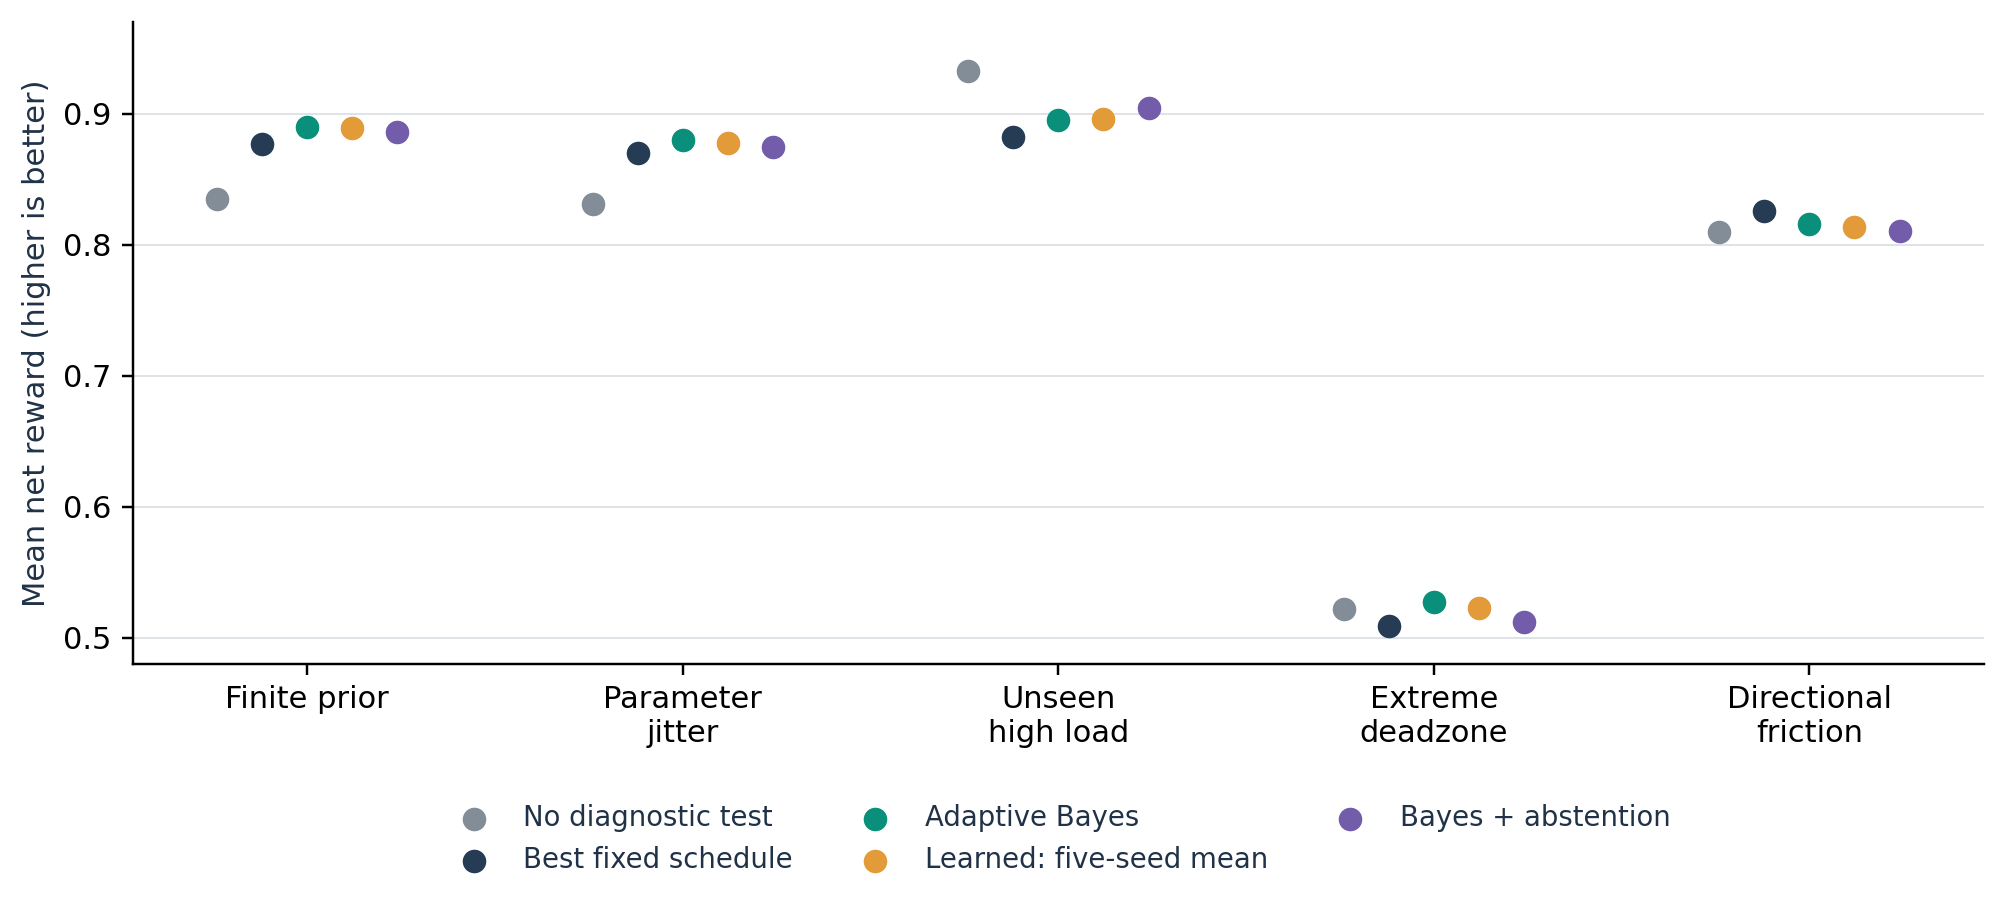
\includegraphics{figures/policy_results.png}
\caption{Mean net reward on 512 shared cases per cohort. The learned
point is the mean of five fitted seeds. Cohorts are separate specified
populations, not a temporal progression.}
\end{figure}

Under the finite prior, Bayes improves on the fixed schedule by
0.012329, with interval {[}0.010389, 0.014152{]}. Its mean terminal
quality is 0.910015 against 0.907108, while mean diagnostic cost falls
from 2.5 to 1.714844. Therefore the reward gain combines quality and
cost effects. The Bayesian policy stops after the first pulse on 237 of
512 cases and uses the reference on 182; its other choices include
stronger or negative pulses.

The five learned finite-test means range from 0.888518 to 0.890010.
Their mean is 0.889164 and sample standard deviation is 0.000572. Every
learned-versus-Bayes paired interval includes zero. This supports useful
observation-dependent behavior in the constructed setting without
establishing learned superiority over the strong classical baseline. A
nonsignificant difference is also not a formal equivalence result.

On finite-prior cases, Bayes exceeds its matched-frequency shuffled
control by 0.024804 in descriptive mean reward at exactly equal
aggregate diagnostic cost. This supports the relevance of assigning
actions to observations, rather than merely learning a favorable global
action mix. The single-permutation result has no inferential confidence
interval.

\begin{figure}
\centering
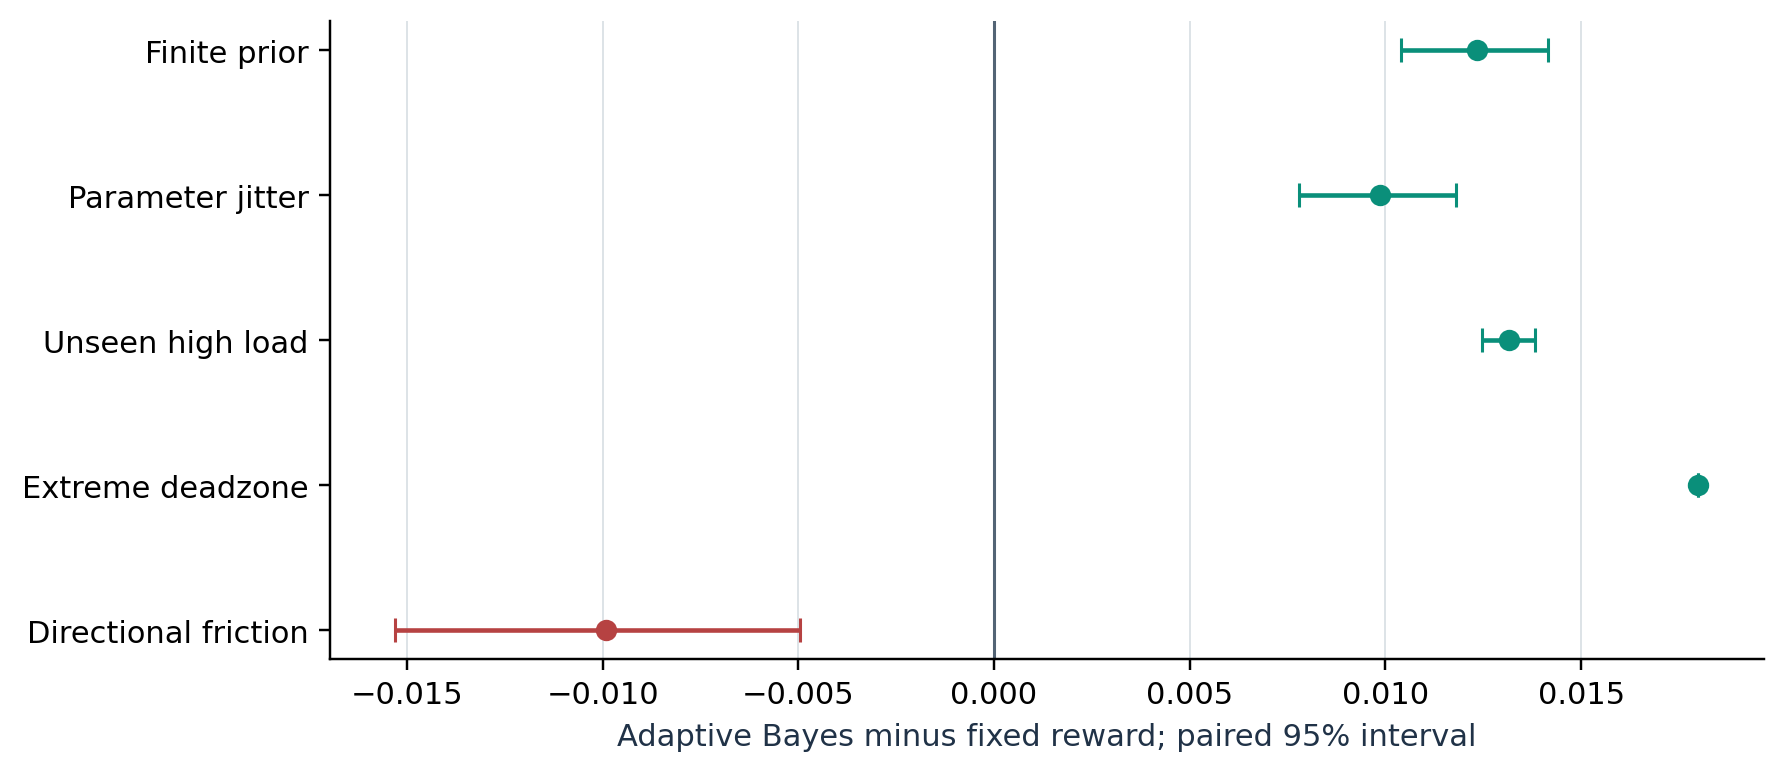
\includegraphics{figures/paired_comparisons.png}
\caption{Paired Bayes-minus-fixed differences and 95\% episode-bootstrap
intervals. The directional-friction result reverses the in-distribution
ordering. The extreme-deadzone difference is entirely a diagnostic-cost
effect in this cohort.}
\end{figure}

The high-load result demonstrates a different failure. No diagnostic
test scores 0.932925, versus 0.895317 for adaptive Bayes. Bayes minus
no-probe is -0.037608 with interval {[}-0.039691, -0.035485{]}. The
fallback improves Bayes to 0.904224 but remains below the no-probe
control. Its flag rate is 34.77\%, leaving many high-load cases
unflagged. A first-measurement mismatch threshold does not reliably
establish that the chosen model is adequate.

Under directional friction, the selected fixed schedule scores 0.825827
against Bayes at 0.815906. Bayes-minus-fixed is -0.009921, interval
{[}-0.015302, -0.004964{]}. The learned mean is lower still at 0.813475.
Observation-dependent selection can therefore be harmful when a
structural assumption used by the inference model fails.

The extreme-deadzone cohort illustrates why raw quality and cost are
retained. Bayes stops after its first test, giving the same quality as
the fixed schedule while avoiding its reference cost. Two learned seeds
take an unnecessary extra pulse and lose exactly 0.012 relative to the
stopping seeds. The fallback worsens the mean to 0.512011, despite
flagging 92.97\% of cases. A high mismatch detection rate alone does not
imply a useful fallback decision.

\subsection{Descriptive inference
cost}\label{descriptive-inference-cost}

A separate timing artifact uses 64 identical saved first observations,
the seed-13 checkpoint, two warmups, and seven repetitions on the shared
CPU environment. Median batch-amortized learned selection including
feature preparation is 5.35 microseconds per case; Bayesian order-15
selection including its posterior is 1,860.88 microseconds. The median
across repeated scalar loops is 73.10 and 2,286.46 microseconds per
call, respectively. Training, model-bank construction, terminal
calibration, and I/O are excluded from both measurements.

These values describe these implementations on an AMD EPYC 7763
environment with NumPy 2.3.5 and its recorded OpenBLAS configuration.
They are not worst-case latency guarantees or a general speed benchmark.
The two policies agree on only 67.19\% of that batch's second actions,
so the timing difference does not establish equal decision quality. Its
practical implication is limited: amortizing diagnostic selection may be
computationally useful, but policy quality and model adequacy remain
separate questions.

\section{Separate physical-unit model and data
path}\label{separate-physical-unit-model-and-data-path}

The SI model represents a single hinged hatch with two identical struts.
It uses illustrative repository CAD mounts, assumed mass and inertia, a
linear force-length relation, a fixed absolute-temperature multiplier,
Coulomb friction and stiction, viscous damping, bounded actuator force
with first-order lag, and inelastic hard stops. It is not used to
generate the normalized benchmark scores.

For hinge angle \(q\), strut length \(L(q)\), inertia \(J\), motor force
\(F_m\), and gas force \(F_g\) per strut, the model uses

\[J\ddot q=2(F_m+F_g)L'(q)-mgr_c\sin(q+q_c)-\tau_{ext}
-\tau_{friction}-2c_s[L'(q)]^2\dot q.\]

The moment arm is the analytic derivative of pin-to-pin length. The
controller uses nominal feedforward and position/velocity feedback. A
changed plant does not silently change its feedforward model; identified
controller parameters must be supplied separately. No electrical
current, battery energy, backlash, flexible-body dynamics, obstacle
contact, or anti-pinch performance is modeled.

The integrator uses an analytic motor-lag update, midpoint geometry and
torque prediction, a dissipative friction projection, and an
average-velocity position update. Switching and damping generally limit
overall accuracy to first order. It shortens the final step to the
requested time and splits at power-loss events. A configured speed
breach terminates the simulation with an explicit event. Detection at
recorded states does not constitute a continuous-time safety guarantee.

\begin{figure}
\centering
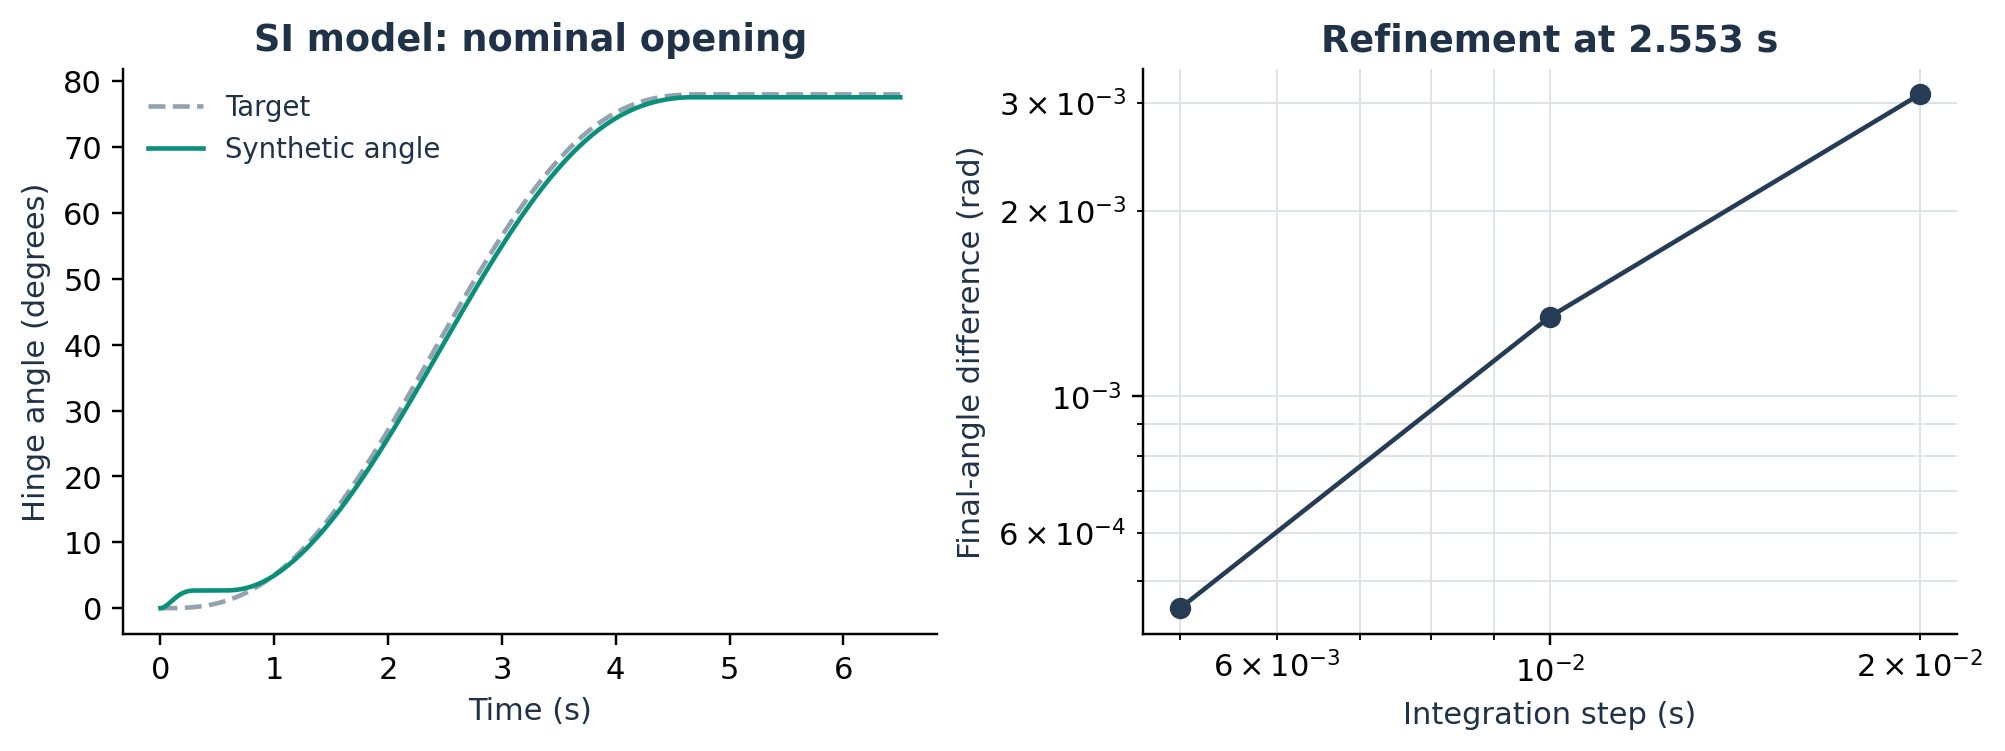
\includegraphics{figures/physical_model.png}
\caption{Separate SI model: nominal synthetic opening and
step-refinement comparison. The reference for the right panel is a 2.5
ms numerical run at the same 2.553 s final time, not a measured
trajectory.}
\end{figure}

Numerical checks give a maximum mount-derivative discrepancy of
\(4.90\times10^{-11}\) m and a constant-force virtual-work residual of
\(6.86\times10^{-7}\) J. Final-angle differences from the 2.5 ms
reference at 2.553 s are 0.003094, 0.001346, and 0.000452 rad for 20,
10, and 5 ms steps. In a separate frictionless contact-free case, energy
drift decreases from 0.013779 J at 20 ms to 0.000215 J at 2.5 ms. These
checks establish implementation consistency and refinement behavior for
the tested cases, not physical accuracy.

The nominal opening simulation completes 6.5 s with tracking RMSE
1.07157 degrees. At 78 degrees, the assumed struts produce 68.85 Nm of
opening torque against 134.60 Nm of closing gravity torque. After the
assumed 8 Nm static-friction capacity, 57.75 Nm of additional holding
capacity is required. The default unpowered case falls and reaches its
configured speed limit after 0.27 s. An explicitly modeled 70 Nm holding
brake prevents drift in that synthetic case. It is an architecture
change, not evidence of a real brake.

The NHTSA investigation of Toyota Sienna power liftgates documents one
architecture in which the motor disengages at full opening and gas
struts provide support (National Highway Traffic Safety Administration
2008). It motivates this architecture-dependent hold test. Its measured
values are not used as labels for RecursiveCal's different geometry, and
it does not imply that every powered liftgate must rely on gas struts
alone.

The implemented data path accepts strict SI CSVs with source
declarations and file hashes. A force curve is fit on explicit training
rows, evaluated on separate validation rows, and applied to geometry
only within its observed training-length range. Trajectory comparison
interpolates a saved simulation at observed timestamps without
refitting, time alignment, or extrapolation. Optional acceptance
thresholds are recorded; without a threshold, the result is unevaluated
rather than a fabricated pass.

\begin{figure}
\centering
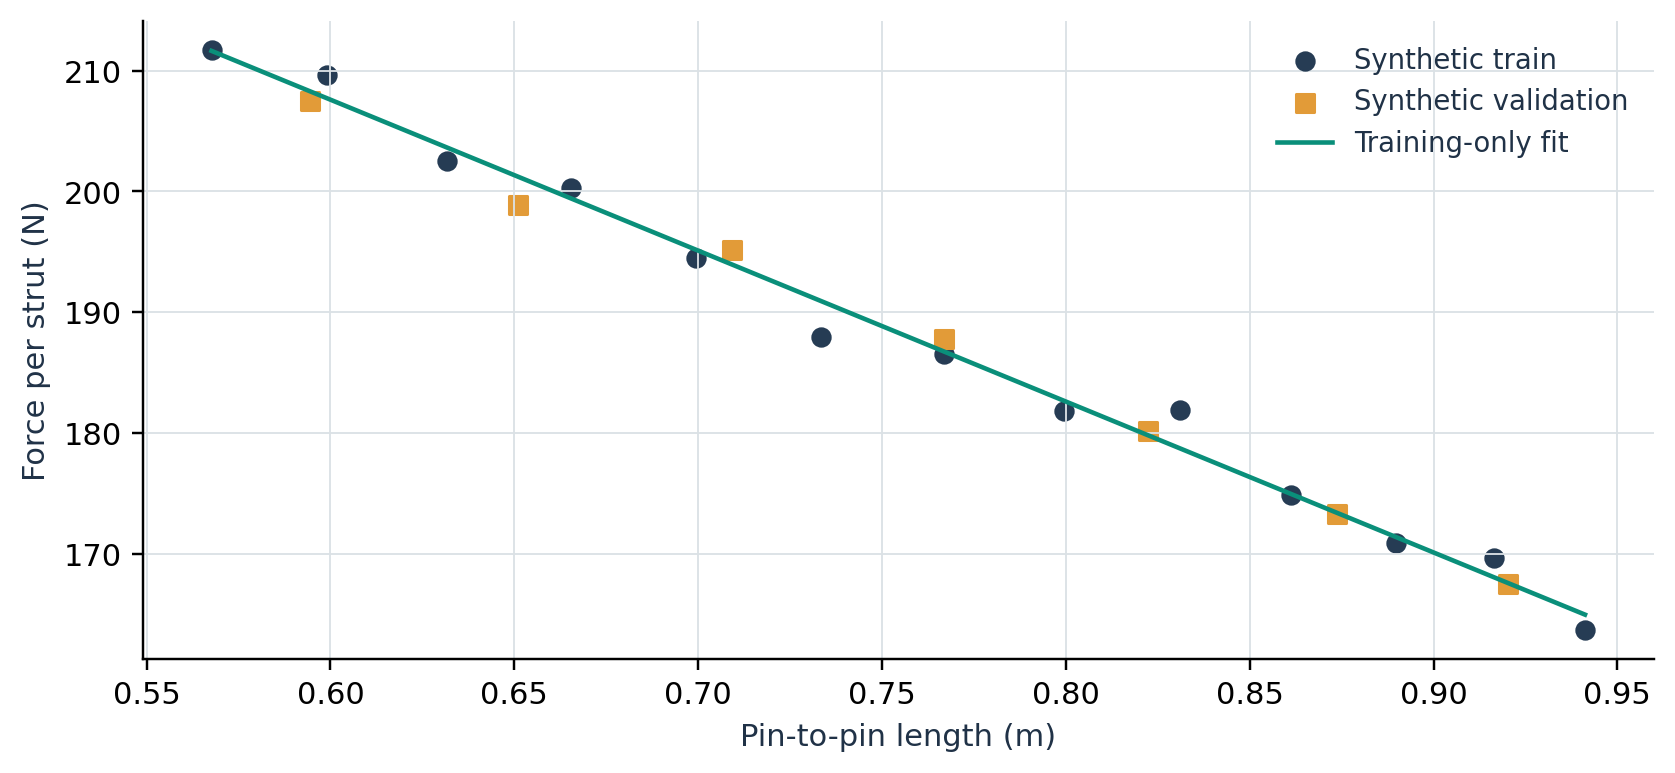
\includegraphics{figures/force_fit.png}
\caption{Synthetic force-fit workflow: 13 training and seven held-out
rows. These values were generated from an assumed force curve and
artificial noise, so their agreement is an ingestion and fitting
demonstration.}
\end{figure}

The included force example has held-out RMSE 1.12368 N per strut. A
separate synthetic trajectory sample has angle RMSE 0.001302 rad against
the simulator. Because both examples share their generating assumptions
with the implementation, neither independently validates physical
behavior. Declaring imported coefficients measured also leaves
subsequent generated motion labeled synthetic.

\section{Software and
reproducibility}\label{software-and-reproducibility}

The MIT-licensed package provides a foreground CLI, loopback-only
workbench API, packaged web assets, simulation and CSV exports,
measurement fitting and replay, experiment execution, and artifact
verification. The browser presents live local calculations separately
from recorded examples. No cloud account, paid API, or GPU is required
for the new suite. Historical optional Torch and Verifiers paths remain
separate.

The diagnostic release contains 51,200 policy-by-case rows, 2,560
distinct evaluation cases, five learned checkpoints, train/validation
arrays, saved observations, selection records, protocol bytes, and
source/runtime hashes. The verifier reconstructs aggregate results,
checks paired identities and finite values, and replays learned choices
from saved observations. Hash verification protects integrity but is not
an independent scientific replication.

The frozen scalar benchmark and historical CAD simulator remain
unchanged. Earlier result JSONs are preserved. Repaired historical
entrypoints have explicit paths and corrected duration accounting; the
historical low-pulse rounding behavior remains documented. The new SI
model uses a separate identifier and does not retroactively change old
scores.

Unit and integration tests cover model equations, geometry identities,
refinement, data validation, held-out fitting, policy information
boundaries, model shifts, checkpoint replay, artifact corruption, CLI
behavior, and real HTTP requests. Browser acceptance tests cover
interactive calculations, export, fitting and application, replay, error
handling, recorded mode, and responsive layout. CI checks clean wheel
installation against supported Python and NumPy versions. Software test
success is kept distinct from the deliberately failing default
passive-support condition.

\section{Limits and publication
scope}\label{limits-and-publication-scope}

The finite hypothesis bank, fixed first probe, two-stage horizon,
discrete calibration grid, and designed noise model make classical
inference particularly strong. The learned policy shares a Bayesian
terminal calibrator and posterior features. Its results do not show that
a model-free method independently learned physical identification or
low-level control.

The benchmark's original numerical timing remains imperfect: a
0.55-second low pulse becomes 0.56 seconds at a 20 ms step. Its
equations are frozen for reproducibility, while the separate SI model
implements exact final duration. Future changes to benchmark timing
require a new model version and complete reevaluation. The present
numerical limitations are part of the result, not concealed by a new UI.

Model misspecification is only sampled through a few specified synthetic
shifts. The mismatch statistic has no distribution-free coverage or
regret guarantee, and its prior-optimal fallback can be harmful.
Stronger conclusions would require a broader benchmark designed
independently of these results, more training seeds where relevant, and
an independent replication.

No hardware measurements were acquired, no physical I/O adapter was
implemented, and no vehicle was controlled. Physical accuracy, transfer
of the normalized learned policy to the SI model, anti-pinch safety,
real-time hardware-in-the-loop operation, and certification remain
unestablished. The released measurement protocol defines the independent
acquisitions and held-out comparisons needed to support a later physical
claim. Those evidence requirements cannot be satisfied by additional
synthetic runs alone.

\section{Conclusion}\label{conclusion}

RecursiveCal is an executable workbench for studying diagnostic
selection while keeping implementation, statistical evidence, and
physical validity distinct. Adaptive policies improve the deliberately
constructed finite-prior task, yet a structural friction change makes a
fixed schedule better. The learned contextual bandit is competitive in
the narrow synthetic setting without an established advantage over
Bayesian experimental design. A separate SI mechanism and data-ingestion
path expose support failures and numerical assumptions rather than
treating a plausible visualization as validation. The release provides
inspectable code and artifacts for further research, with the limits of
each claim stated alongside its evidence.

\section{Availability}\label{availability}

Repository: \url{https://github.com/Venkat-RJ/RecursiveCal}. The exact
files used are under \texttt{research/releases/v0.3},
\texttt{research/releases/physical-v1}, and
\texttt{research/releases/inference-v0.3}. The experiment manifest and
audit record source hashes. Figures are generated by
\texttt{scripts/build\_paper.py} from those artifacts. This document is
a working draft for author review and has not been submitted to a venue
or independently peer reviewed.

\section{References}\label{references}

\phantomsection\label{refs}
\begin{CSLReferences}{1}{0}
\bibitem[\citeproctext]{ref-agarwal2021}
Agarwal, Rishabh, Max Schwarzer, Pablo Samuel Castro, Aaron Courville,
and Marc Bellemare. 2021. {``Deep Reinforcement Learning at the Edge of
the Statistical Precipice.''} In \emph{Advances in Neural Information
Processing Systems}. Vol. 34.
\url{https://proceedings.neurips.cc/paper_files/paper/2021/hash/f514cec81cb148559cf475e7426eed5e-Abstract.html}.

\bibitem[\citeproctext]{ref-nhtsa2008}
National Highway Traffic Safety Administration. 2008. {``Engineering
Analysis Report: EA06-020, Toyota Sienna Power Liftgates.''} U.S.
Department of Transportation, Office of Defects Investigation.
\url{https://static.nhtsa.gov/odi/inv/2006/INCR-EA06020-29305P.pdf}.

\bibitem[\citeproctext]{ref-patterson2024}
Patterson, Andrew, Samuel Neumann, Martha White, and Adam White. 2024.
{``Empirical Design in Reinforcement Learning.''} \emph{Journal of
Machine Learning Research} 25 (318): 1--63.
\url{https://jmlr.org/papers/v25/23-0183.html}.

\end{CSLReferences}

\end{document}
